\documentclass{article} % For LaTeX2e
\usepackage{nips13submit_e}
\usepackage{hyperref}
\usepackage{url}
%\documentstyle[nips13submit_09,times,art10]{article} % For LaTeX 2.09
\usepackage{pifont}
\usepackage{times,amsmath,color, balance,tabularx,caption,
amssymb,graphicx,epsfig,cite,psfrag,subfigure,multirow,cases,algorithmic,mathtools}
\usepackage{longtable}
\usepackage{booktabs}
\usepackage{adjustbox}
\usepackage[ruled,vlined]{algorithm2e}

\newtheorem{claim}{Claim}
\newtheorem{guess}{Conjecture}
\newtheorem{definition}{Definition}
\newtheorem{fact}{Fact}
\newtheorem{assumption}{\underline{Assumption}}
\newtheorem{theorem}{\underline{Theorem}}
\newtheorem{lemma}{\underline{Lemma}}
\newtheorem{ctheorem}{Corrected Theorem}
\newtheorem{corollary}{\underline{Corollary}}
\newtheorem{proposition}{Proposition}
\newtheorem{example}{\underline{Example}}
\newtheorem{remark}{\underline{Remark}}
\newtheorem{problem}{\underline{Problem}}
\def\Ei{\mathop\mathrm{Ei}}
\def\E{\mathop\mathrm{E}}
\def\tr{\mathop\mathrm{tr}}
\newcounter{mytempeqncnt}

\title{Decoding Team Composition in MOBA Games \\ A Learning Approach}


\author{
Jiachen Li$^*$, Yilin He$^\dag$, and Chengliang Lian$^*$\\
Language Technologies Institute$^*$ and Machine Learning Department$^\dag$ \\ School of Computer Science \\
Carnegie Mellon University, Pittsburgh, PA, 15213 \\
\texttt{\{jiachenl, yilinhe, clian\}@andrew.cmu.edu}
}

% The \author macro works with any number of authors. There are two commands
% used to separate the names and addresses of multiple authors: \And and \AND.
%
% Using \And between authors leaves it to \LaTeX{} to determine where to break
% the lines. Using \AND forces a linebreak at that point. So, if \LaTeX{}
% puts 3 of 4 authors names on the first line, and the last on the second
% line, try using \AND instead of \And before the third author name.

\newcommand{\fix}{\marginpar{FIX}}
\newcommand{\new}{\marginpar{NEW}}

\nipsfinalcopy % Uncomment for camera-ready version

\begin{document}


\maketitle

\begin{abstract}
Team composition of massive online battle arena (MOBA) games has become an interesting as well as challenging problem studied by many researchers and companies. In the setting of MOBA games, good team compositions will improve the chance of winning, while bad team compositions might ruin your game. \\
In this project, we applied machine learning method to analyze the impact of team composition on the MOBA game result. We collected data from two most popular MOBA games: DotA 2 and LoL. We proposed two feature models in representation of data and compared algorithms with different characteristics such as Logistic Regression (LR), Support Vector Machine (SVM) and Deep Belief Networks (DBN) which are used to train the predicting model. At last our results proved that the team composition could, to some degree, predict the winning of games and we gave further analysis to the intrinsic relationship of the results.
\end{abstract}

\section{Introduction}


%\begin{center}
%   \url{http://papers.nips.cc}
%\end{center}

Multiplayer online battle arena (MOBA) is a rising force in online games that has features of fast paced, single round and team play. In the past few months, more than 27 million players fight with each other per day in one of such kind of game called League of Legends (LoL)\cite{Ian} while millions are attracted by another game called Defense of the Ancient 2 (DotA2). International MOBA tournaments are held over the world with a prize pool of over \$10 million\cite{Valve}.  Analysis on MOBA games will not only gain us experience of data analysis but will also be beneficial to players and game companies all over the world.

In MOBA games like LoL or DotA 2, two groups of five players are pitted against each other based on their levels of game proficiency. In the beginning of a game, each player first picks an unique character out of over 100 options, and these 5 characters picked in a group finally forms a team. There are many common strategies for picking characters that gives a good team composition.Players control selected characters to battle for victory. A typical game would last 30-60 minutes.

There are many factors which influence end game results. Player's skill, team composition and in-game strategy are some important aspects of MOBA game play. Although intuitively individual player��s skill might sounds like the biggest factor of their chance of winning, it is not true because game system are designed to match players with similar skills with each other. As a result, team composition and in-game strategy plays a much more important role in deciding the game outcome

In this paper, we are interested in analyzing the impact of team composition on game outcome. How to form a good team composition to achieve highest winning probability is always an interesting questions to the online communities as well as professional teams.
The challenging part for this problem is the large number of possible team compositions. To be specific, since there are generally more than 100 characters for players
to choose, the number of possible team compositions for both teams are more than $\binom{100}{10}\cdot\binom{10}{5}\approx 4\times 10^{15}$.

To answer this question, we can transform it into a classification problem in machine learning: given a team composition, predict the result for the game. With this problem transformation, we can learn how to form a good team composition by interpreting the learning model parameters and then form good team composition in practice by using the learned model for prediction and recommendation.

The goal of this project is to achieve more than 60\% accuracy on the prediction. The prediction accuracy is limited by the nature of this problem. Achieving over 80\% accuracy implies that most of the game are determined in the character picking stage, which mean the following 30-60 minutes of actual game play have very little influence on the result. This is undesirable for the player. Therefore despite the fact that team composition is an important factor for end game result, our prediction shouldn't be too high.


%\subsection{Related Work}
%Conley and Perry have previously worked on predicting win ratio based on heroes picked by the team in DotA 2. In their work, they have reported 69\% accuracy using logistic regression and K-NN.

%\subsection{Organization of this Report}
%The remaining of this report is organized as follows: Section II presents the collection of the data set, Section III introduces the learning model and assumptions ..



\section{Data Set Preparation}
We have obtained two data sets for this study, one from the LoL and the other from DotA 2. The whole dataset contains more than 80,000 independent game history records in total, which are adequate for this project.

\subsection{Data Collection}

The dataset was collected through public APIs provided by the video game producers Riot and Steam respectively. The APIs can provide us with a given number of most recent completed games as well as the corresponding whole statistics. To make full use of the APIs, we ran our feature collection program on AWS Cloud Computing resources to collect these data in a $7\times24$ manner.


\subsection{Data Contents}

The contents of the original data collected from APIs are shown as follow:


\begin{itemize}
\item \textit{Game Id}: An Unique identifier for the game, used to avoid data redundancy;
\item \textit{Game duration}: how long the each game last, used for data cleaning;
\item \textit{Winner}: The winning team, used as labels;
\item \textit{Team composition}: the characters selected by each team, used as main features;
\item \textit{Skill levels}: the player's performance in his/her past history, used to evaluate the potential performance of this player;
\item \textit{KDA Statistics}: the character's performance in this game, i.e., how many other characters it killed (K), how many times it died (D) and how many times it assisted its teammate to kill the other characters (A).
\end{itemize}

\subsection{Data Cleaning}

As we all known that the performance of machine learning algorithms is heavily dependent on the quality of features. So before extracting features from raw data, we need to do some data cleaning.

Since the public APIs always return the most recent game records, we should first to check whether there is any redundancy in our data set. Besides, we need to make sure the data is useful, which can be verified from the game duration. For example, if the game duration is too short, then it is quite possible that some player leaves the game early, so that this record may not be able to support our learning goal and should be dropped. Finally, we will have a look at the KDA statistics, if some character's KDA is below a normal level, then this character may not fully participate into the game. Therefore, the corresponding record should also be dropped.

After finishing these procedures, we can then extract features from the data and train our models.



\section{Models and Assumptions}

In this section, we proposed two models for decoding team composition. The first ``Character Ranking Model'' analyzes the team composition by ranking the importance of each character in the team, while the second ``Predicting Model with Prior'' takes the characters' prior knowledge such as the player skill level and the winning probability between different characters into consideration. The first model can be used to interpret the parameters while the second model is mainly used to improve the predicting performance.

\begin{figure}[t]
  \centering
    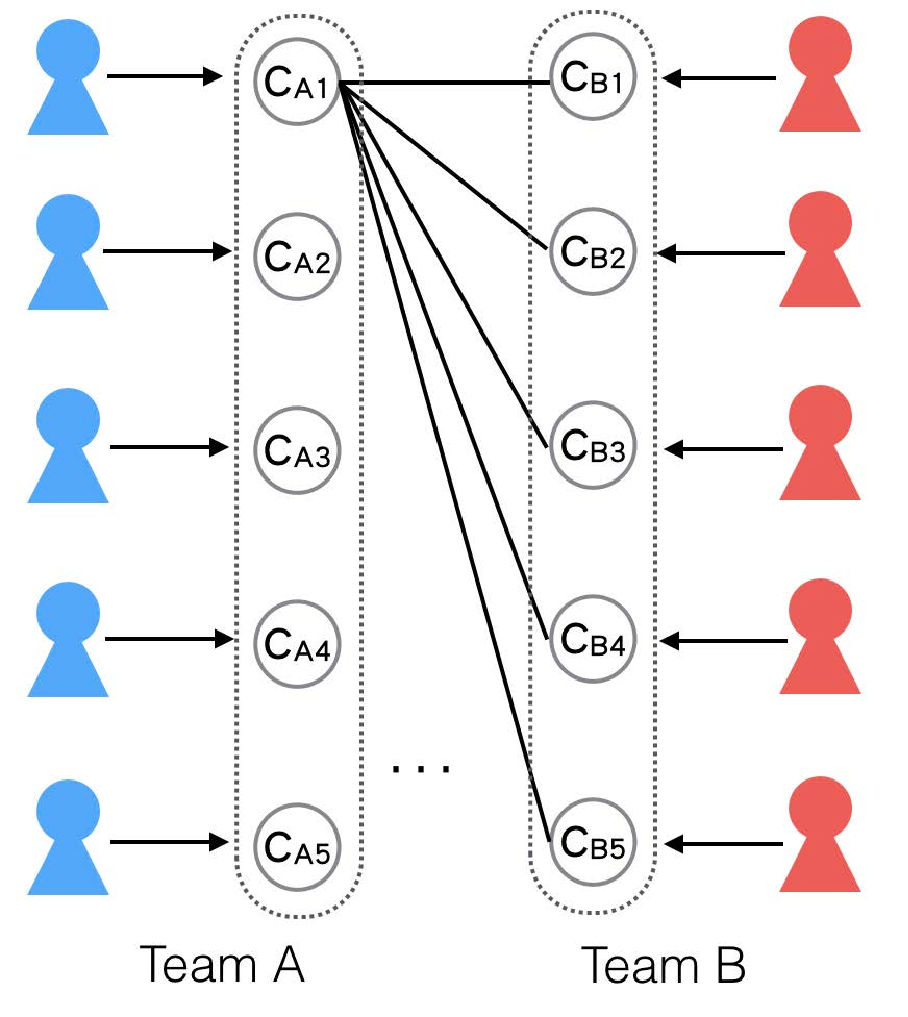
\includegraphics[width=60mm]{team_comp.pdf}
  \caption{An illustration of team composition and the aspects that may influences the game result.}
  \label{fig:team_comp}
\end{figure}



To start discussing the models,  as shown in Fig. \ref{fig:team_comp}, let's first define the two teams in the game as team $\mathcal{A}$ and team $\mathcal{B}$, where each team contains five unique characters (i.e., $c_{A1},\ldots,c_{A5}$ for team $\mathcal{A}$ and $c_{B1},\ldots,c_{B5}$ for team $\mathcal{B}$). Moreover, suppose that the game has $N$ different characters in total, then all the characters can be encoded with an integer from $1$ to $N$.

\subsection{Model-I: Character Ranking Model}

In the character ranking model, the characters in each team are encoded as some kind of indicator vector, and what we really want to learn from this model is the corresponding weights for different characters in the machine learning algorithms, specially the one with a linear decision boundary, which measures how important the characters to a team. To introduce the that, we may first need to make some assumptions:

\begin{assumption}
We assume that players in both team all have high skills. Moreover, they are proficient with the characters they pick.
\end{assumption}

\begin{remark}
This assumption is reasonable because we only collected the records of players with
higher skill levels during the data collection part. Moreover, in order to win the game, the players are not likely to pick the characters that they are not familiar with.
\end{remark}

With this assumption, we can further assume that the game result is independent of the players, then we can use the vector $\textbf{x}=\{x_1,x_2,\ldots,x_N\}$ to represent the training feature. The element $x_i$ indicates the presence of $i$th character in the game, and the value for it is given by

\begin{equation}
x_i =
\begin{cases}
1 &  \text{if $i\in \mathcal{A},$} \\
-1 &  \text{if $i\in \mathcal{B},$} \\
0 & \text{otherwise.}
\end{cases}
\end{equation}

Besides, the team that win the game will serve as the label for the corresponding feature.


\subsection{Model-II: Predicting Model with Prior}


Unlike the character ranking model where we make the independent assumptions between
player skills and game results. This predicting model takes the relationship of different characters into account, and let it work as the prior information. For example, Fig. \ref{fig:team_comp} has shown the factors that may have potential influence on the game result. It can be seen from the figure that the performance of one specific character should have connections with all the other characters in the opposite team. This is not difficult to understand because there are many times in the game that all the characters in a team will need to work together to achieve their goals. Therefore, to learn the team composition, we need also use such information.

To utilize these additional information, we first introduce the character matrix.
\begin{definition}
A matrix $C \in \mathbb{R}^{N\times N}$ is called the character matrix if the element $c_{i,j}$ indicates the probability that the team with character $i$ beats the team with character $j$, i.e. $c_{i,j}=\text{Pr}\{\text{team with character $i$ wins when played against team with $j$}\}$.
\end{definition}

The character matrix can be computed from the statistics of game history and it gives us an character performance evaluation between different character pairs that can be used for learning. Based on that, we introduce the following model. For each team, we have two feature vectors. Let's take team $\mathcal{A}$ as an example, the feature vectors can be defined as:
\begin{equation}
\mathbf{a}=\{a_1,a_2,\ldots,a_N\} \ \ \ \ \ \ \ \ \ \ \ \ \ \ \ \
\mathbf{a'}=\{a_1',a_2',\ldots,a_N'\},
\end{equation}
where the elements are defined as:
\begin{equation}
a_i =
\begin{cases}
1 & \text{if $i\in\mathcal{A}$}\\
0 & \text{otherwise}
\end{cases}\ \ \ \ \
a_i' =
\begin{cases}
\prod_{j\in \mathcal{\bar{A}}} c_{i,j} & \text{if $i\in\mathcal{A}$} \\
0 & \text{otherwise}
\end{cases}
\end{equation}

The feature vector $\mathbf{a}$ shows the characters chosen in team $\mathcal{A}$, while the feature vector $\mathbf{a'}$ indicates the ``likelihood'' that team $\mathcal{A}$ with character $c_{Ai}$ beats team $\mathcal{A}$, where the $c_{i,j}$ is the element from character matrix $C$.

After obtaining the similar two feature vectors for team $\mathcal{B}$ (i.e., $\mathbf{b}$ and $\mathbf{b'}$), we can then build the modified feature vector for this model, which is $\textbf{x}=\{\mathbf{a},\mathbf{a'},\mathbf{b},\mathbf{b'}\}$.

\begin{remark}
Note that in the midway report we proposed a feature matrix $F \in \mathbb{R}^{N\times N}$ and wanted to utilize players information (i.e., use a function $g(P_{\mathcal{A},i},P_{\mathcal{B},j})$ to evaluate the winning ratio between two players) to enhance the feature. The element of feature matrix $F$ is designed as
\begin{equation*}
f_{i,j}=c_{i,j} \cdot g(P_{\mathcal{A},i},P_{\mathcal{B},j}),
\end{equation*}
where the $c_{i,j}$ is the element from character matrix, $g(P_{\mathcal{A},i},P_{\mathcal{B},j})$ is the function that measure the winning ratio between the player in group $\mathcal{A}$ using character $i$ and the player in group $\mathcal{B}$ using character $j$.

However, our work after midterm showed that this approach is not available. The main difficulty is to found a reasonable way to do dimensionality reduction. We have tried to use the characters' KDA statistics to cluster them into several groups, but the results suggest that the differences between each two group are quite small, which means that characters didn't have clear patterns over the KDA statistics. This is reasonable since the KDA statistics are greatly influenced by players' in game performance, so that even for the same character, different players may lead to totally different KDA. Besides, due to the privacy policy, we may be not able to get the skill levels for all the players. Then if we which makes the evaluation becomes difficult.
\end{remark}

Compared with the feature matrix idea, this feature model takes a more compact way to utilize the features (e.g. convert the character to characters relationship to character to team relationship through the winning ``likelihood''). Though this may lose some information about the exact relationship, this modified feature only has a dimension of $4\times N$, which is only 4 time larger than that of character ranking model, so it doesn't have the high dimension problem and is eligible for training.


\section{Evaluation and Discussion}

In this section, we apply our feature models to different machine learning algorithms, train different learning models and use them to achieve our goals such as evaluation of convergence, parameters interpretation, game result prediction and character recommendation.

The feature using Character Ranking Model in the experiments is denoted as ``w/o Prior'' while the feature using Predicting Model with Prior is denoted as ``w/ Prior''. In general, we used $80\%$ of the whole data set as the training data, the other $20\%$ as the test data. And the detailed algorithm parameters setting are introduced as the Game Result Predicting part.

\subsection{Evaluation of Convergence}


\begin{figure}[t]
  \centering
    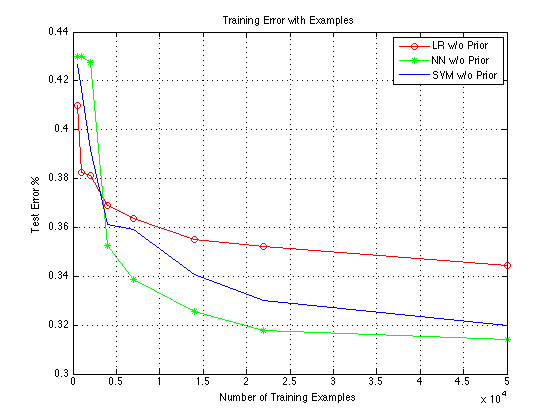
\includegraphics[width=90mm]{resWOprior.png}
  \caption{The test error versus number of training data for Character Ranking Model}
  \label{fig:error_without_prior}
\end{figure}


\begin{figure}[t]
  \centering
    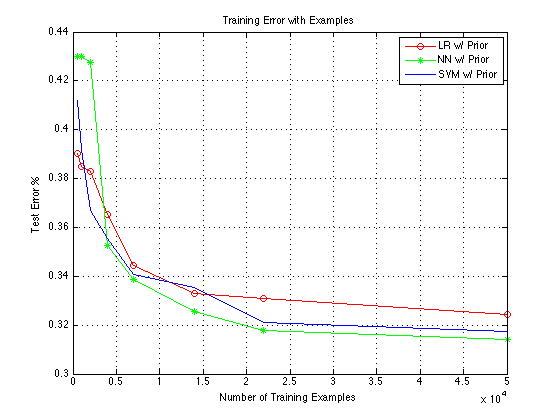
\includegraphics[width=90mm]{withPrior.png}
  \caption{The test error versus number of training data for Predicting Model with Prior}
  \label{fig:error_with_prior}
\end{figure}

The first part of the evaluation is about the convergence of different algorithms over different training data size, which can be used to check whether our collected data sets are large enough for this learning task.

It can be seen from Fig. 2 and 3, as we increase the training data, the error rate of different algorithms converge quickly at first and then become much stable when the number of training data is larger than $25,000$, which can be regarded as a threshold that determines whether the data size is able to make some meaningful results. Besides, comparing the results between Fig.2 and 3, we can see that the learned model with features contain prior knowledge converges better, which gives us a hint that our Predicting Model with Prior may work better.




\subsection{Parameter Interpretation}

\begin{figure}[t]
  \centering
    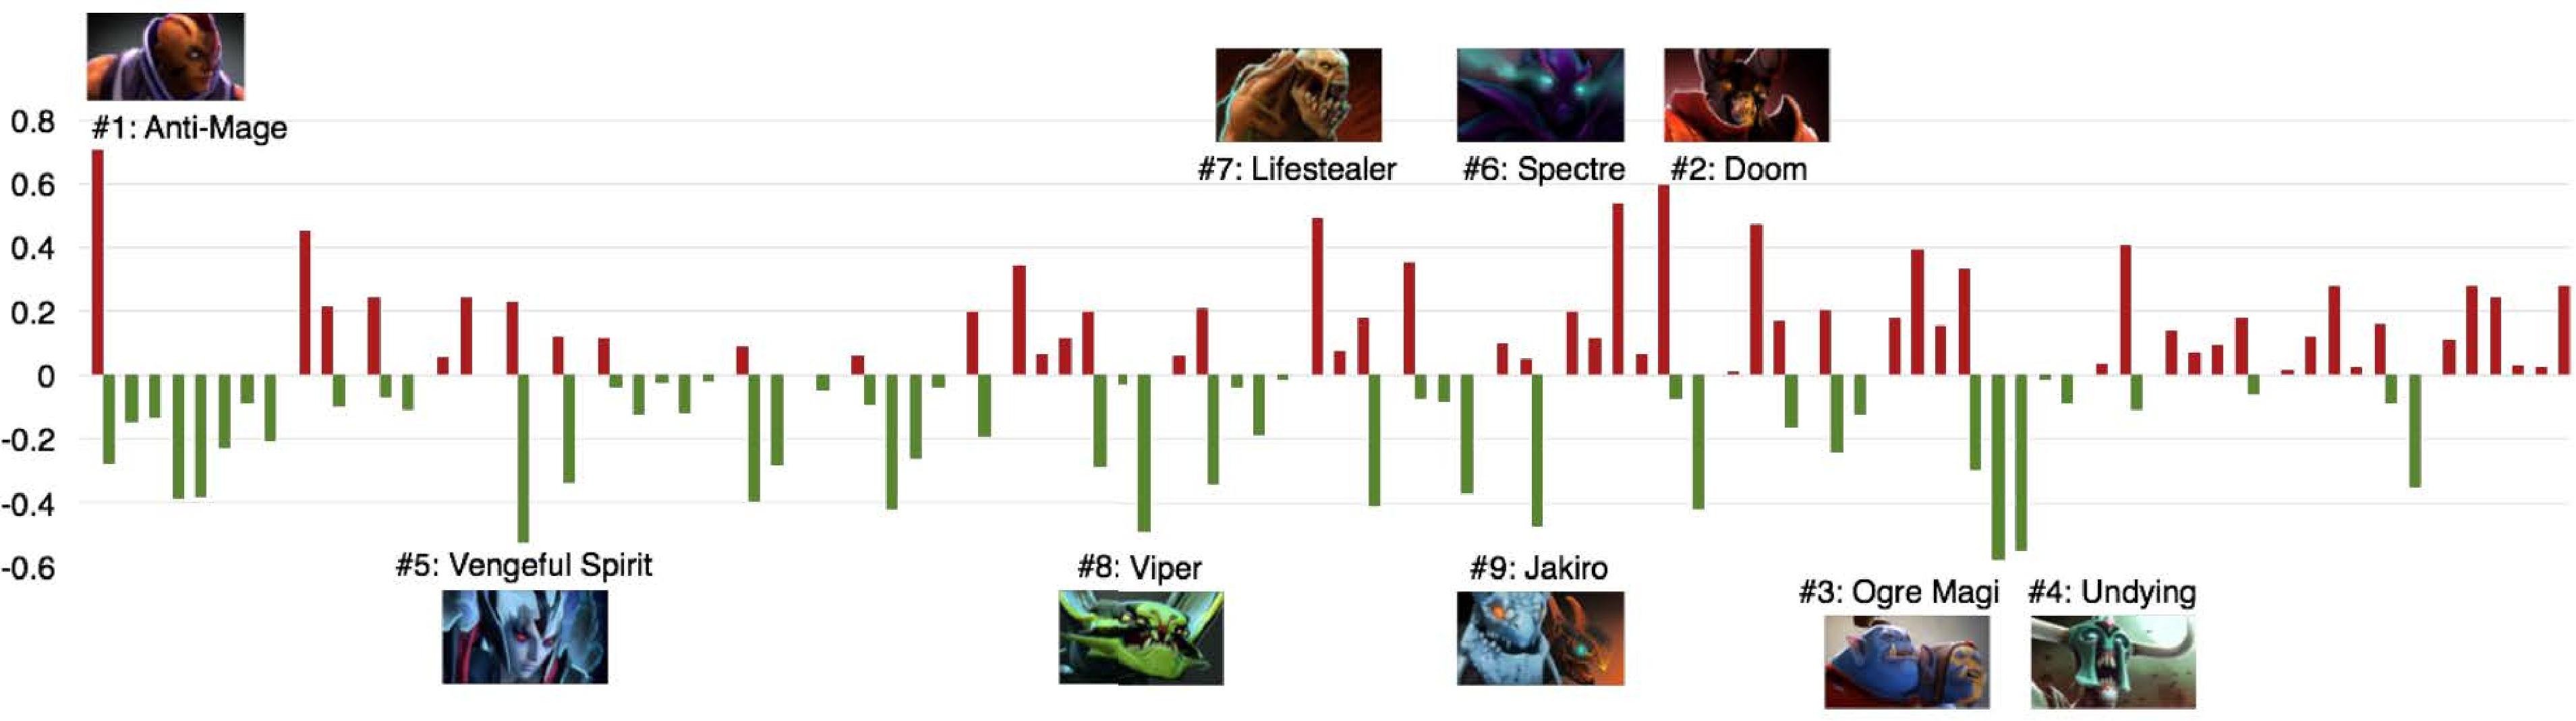
\includegraphics[width=125mm]{params.pdf}
  \caption{Visualization of linear model parameters using Character Ranking model.}
  \label{fig:params}
\end{figure}

If we use the machine learning algorithms that have a linear decision boundary for classification (e.g., Logistic Regression and linear kernel SVM), the parameters (e.g., $\mathbf{\beta}$) of the learned linear decision boundary (e.g., $f(\mathbf{X}) = \mathbf{\beta}\times \mathbf{X}$) will have a direct meaning under the Character Ranking model, i.e. each weight we get for the corresponding character implies how this character could have impact on the final games result. In other words, it means that how important that this character for the team!

Fig. 4 shows an example of parameters visualization from Logistic Regression using Character Ranking model. The weight vector we obtained can represent each character's influence on game result. For character $i$, a positive (red) weight implies that picking this character will increase the chance of winning, while a negative (green) weight indicates that picking this character may decrease your chance for winning. Since we want to do prediction by ranking the importance of different characters, we do not consider synergy between characters. Therefore, during the prediction phase, given 2 teams that are comprised of different characters, we could expect the team with more dominant larger weights wins the game.

\begin{remark}
If you are familiar with DotA 2, you may find that the characters with high ranks are exactly the core players in the games based on players experiences, which, from another perspective, shows that our learned ranking is reasonable and our feature model is correct.
\end{remark}




\subsection{Game Result Prediction}

\subsubsection{Parameters setting}

The logistic regression is implemented by maximizing the log-likelihood, the optimization algorithm used is gradient descent. The learning rate is set as 0.003 while the iteration times for each run is taken as 100. The report value is the average over multiple runs (e.g., 20).

The SVM is implemented based on the LIBSVM library [?], and we used the Gaussian Kernel for our classification problem. 

The Deep Belief Network (DBN) is implemented based on the DeepLearnToolBox developed by [?], we used a 3 hidden layers DBN with sigmoid unit, the learning rate for neural network is taken as 0.001, the number of epochs for pre-training is 10 while the number of epochs for fine-tuning is 100. The output layer is ``softmax''.



\subsubsection{Results Analysis}
\begin{table}[ht]
\center
\captionsetup{font={small}}
\caption{Prediction result of different algorithms}
\begin{tabular}{|c |c |c |c |c |}
\hline
Algorithm & \multicolumn{2}{c|}{DotA 2}    & \multicolumn{2}{c|}{LoL}   \\
\hline
Accuracy (\%) & w/o prior   & w/ prior  & w/o prior  & w/ prior  \\ \hline
Logistic Regression    & 65.57         & 67.58     & 55.90         & 55.36
\\ \hline
SVM(Gaussian Kernel) & 68.02 & 68.24 & 55.97 & 56.45
\\ \hline
Deep Belief Networks  & 67.30  & 68.60   & 56.10 & 56.80     \\ \hline
\end{tabular}
\end{table}



In neural networks model, we choose to use 3 layers: 1 hidden layer with 100 nodes. The input layer has p nodes and the output layer has 2 nodes. We implemented feedforward back propagation neural network. Sigmoid transform was applied and lambda in cost function was set to 0.5. (Since the evaluation of error probability versus the number of sample is too expensive for neural networks, we didn't do that in this midway report, but we will add it in the final report)

While we can not directly interpret the parameters we obtained from neural networks model, the high accuracy shows the importance of considering the relationship between selected characters. Since logistic regression has a linear decision boundary, it can only make prediction based on a linear combination of individual characters. Therefore, logistic regression can not capture the relationship between selected characters. On the other side, the learning process of Neural Network combines input feature in the hidden layer to take consideration of the relationship between selected characters.

\subsubsection{Advanced Discussion}

\begin{table}[ht]
\center
\captionsetup{font={small}}
\caption{Prediction result of regularized logistic regression}
\begin{tabular}{|c |c |c |c |c |}
\hline
Algorithm & \multicolumn{2}{c|}{DotA 2}    & \multicolumn{2}{c|}{LoL}   \\
\hline
Accuracy (\%)                       & w/o prior   & w/ prior  & w/o prior  & w/ prior  \\ \hline
LR + L1 penalty  & 67.70 $\pm$ 0.10    & 67.50 $\pm$ 0.11     & 56.30 $\pm$ 0.25  & 56.18 $\pm$ 0.25     \\ \hline
LR + L2 penalty   & 67.68 $\pm$ 0.12   & 67.44 $\pm$ 0.13  & 56.43 $\pm$ 0.22  & 55.18 $\pm$ 0.24 \\ \hline

\end{tabular}
\end{table}
p-value $<$ 2.2e-16 for all values in table 2.
We looked at number of non-zero parameters in L1 regularization and found out that over 90\% of the parameters are non-zero for character ranking model without prior. However, only 50\% of the parameters are non-zero are non-zero.

We ran L1-regularized and L2-regularized logistic regression on both data set using R with LiblineaR package. Package heuristicC was used to calculate cost parameter according to the Joachim's heuristics. During preprocessing, our data was normalized by subtracting mean from each feature and divide it by its standard deviation.
**** cite lib linear and heuristicsC

\subsubsection{Comparison of Data Sets}

Logistic regression yields similar accuracy for LoL and DotA 2 while neural networks has better result on LoL than DotA 2. This result from logistic regression implies that in LoL and DotA 2, selection of individual characters have similar impact on game result. One possible explanation for higher accuracy in LoL data set when using neural networks is that the team composition in LoL focus more on the synergy between characters, thus considering more complicated relationship between characters gives better result.

DotA 2 dataset has more than 60,000 sample data while LoL has 15,000. Our model generally had better performance on DotA 2 than LoL because we collect more training data.




\subsection{Character Recommendation}

The recommendation basically works at two situations: when the opponent has finished teaming up and our team has only 1 character to pick. Under this situation, we could consider teaming up with all the characters left to pick and compute the possibility of winning, using the trained model we have.

On the other situation, if each team is not finished constructing, then we should simply apply the weights we learned from the linear model we constructed. As each weight reflects the overall chance of winning of the character. We could recommend those characters with top weights that has not yet been selected.


\begin{algorithm}[h]
\KwIn{Characters Selected in Two Team $\mathcal{C}$ $\mathcal{C'}$; List of Characters $\mathcal{U}$}
\KwOut{list of the Recommended Character $c$}
{\bf Procedure:} \\

{\bf If:} $\# \mathcal{C'} = 5$  \\
	~~~~~ {\bf For} $x \in \mathcal{U}/\{\mathcal{C,C'}\}$\\
	~~~~~  ~~~~~ $Score(x) = h(\mathcal{C,C'},x$) \\
	~~~~~ {\bf Return} top 5 $c$ of highest $Score(x)$ \\

{\bf Else:} \\
    ~~~~~ {\bf Return} top 5 $c \in \mathcal{U}/\{\mathcal{C,C'}\}$ of highest weight in the model\\

\caption{{\bf Character Recommendation Algorithm} \label{Algorithm}}
\end{algorithm}




\section{Conclusions and Future Work}

\subsection{Conclusions}

In this project, we analyzed the team composition problem in MOBA games through a learning approach. We proposed two feature models, and

First of all, our current results shows that the team composition does have connection with game results and the relationship is encodable.

In addition, we are able to interpret parameters to obtain a better understanding to form a good team composition.

We proposed an algorithm for recommending characters to form a good team composition based on our prediction results.


\subsection{Limitation and Future Work}

    A big limitation of our model is that linear model can not capture the relationship between characters. Therefore we can not explain what leads to a good team composition by analysing synergy between characters. One way to solve this problem is by using the model in Remark 2. However, with $N > 100$, we have over 10,000 dimensions. As as result,the curse of dimensionality make it impossible for us to make a prediction based on this model.

    This leads to some future work for dimensionality reduction. A possible direction of dimensionality reductions is by clustering different characters to several roles. Usually in MOBA games, characters are designed to belong to one or more group such as supportive or aggressive characters. Therefore if we are able to identify the role of each character in the team, we can reduce our dimension from 100+ to <= 10. Originally we plan to cluster based on their KDA statistics which later proven to be invalid. However, clustering based on other attributes such as characters' skill set might leads to a better result.



\subsubsection*{Acknowledgments}


The authors had the great fortune to be instructed by Prof. Gordon and Prof. Singh. We gained much insight of different methods used in machine learning and applied them into our projects. We extend great thanks to our machine learning teach assistant Nicole. Her feedback and comments keeped our project on the right direction. Her idea of applying Lasso on our Logistic Regression model helped us to improve on the prediction result.

We also gave our acknowledgement to Steam and Riot for providing us with comprehensive public API. We give our best respect to these companies for their marvelous games.

\subsubsection*{References}


References follow the acknowledgments. Use unnumbered third level heading for
the references. Any choice of citation style is acceptable as long as you are
consistent. It is permissible to reduce the font size to `small' (9-point)
when listing the references. {\bf Remember that this year you can use
a ninth page as long as it contains \emph{only} cited references.}

\small{

[1] Ian Sherr, ``Player Tally for League of Legends Surges,'' \textit{Digits RSS. N.p., n.d. Web}. 28 Sept, 2014.

[2] Valve, Dota 2 -- 2014 Compendium -- The International. Dota 2 Official Website.

Note that the following part is just for reference!

[1] Alexander, J.A. \& Mozer, M.C. (1995) Template-based algorithms
for connectionist rule extraction. In G. Tesauro, D. S. Touretzky
and T.K. Leen (eds.), {\it Advances in Neural Information Processing
Systems 7}, pp. 609-616. Cambridge, MA: MIT Press.

[2] Bower, J.M. \& Beeman, D. (1995) {\it The Book of GENESIS: Exploring
Realistic Neural Models with the GEneral NEural SImulation System.}
New York: TELOS/Springer-Verlag.

[3] Hasselmo, M.E., Schnell, E. \& Barkai, E. (1995) Dynamics of learning
and recall at excitatory recurrent synapses and cholinergic modulation
in rat hippocampal region CA3. {\it Journal of Neuroscience}
{\bf 15}(7):5249-5262.
}

[ ] Chih-Chung Chang and Chih-Jen Lin, LIBSVM : a library for support vector machines. \textit{ACM Transactions on Intelligent Systems and Technology}, 2:27:1--27:27, 2011. Software available at 
\url{http://www.csie.ntu.edu.tw/~cjlin/libsvm}.

[ ] R. B. Palm, Prediction as a candidate for learning deep hierarchical models of data, \textit{Master's thesis}, Technical University of Denmark (DTU), Informatics, 2012.

[ ] R.-E. Fan, K.-W. Chang, C.-J. Hsieh, X.-R. Wang, and C.-J. Lin. LIBLINEAR: A Library for Large Linear Classification, \textit{Journal of Machine Learning Research} 9(2008), 1871-1874. Software available at \url{http://www.csie.ntu.edu.tw/~cjlin/liblinear}.

\end{document}
